\subsubsection{Listar}

  \paragraph{}Para mostrar esta lista, es necesario establecer la plantilla
  oficial para la que mostrar los cursos académicos disponibles. Para ello,
  habrá que elegir la plantilla en la lista desplegable que se muestra en la
  figura \ref{capturaPantallaSelectPlantillaOficial}.

  \begin{figure}[!ht]
    \begin{center}
      \fbox{
      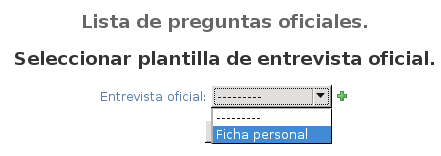
\includegraphics[scale=0.55]{4.Funcionamiento_Aplicacion/4.3.Gestion/4.3.1.Administrador_Principal/4.3.1.19.PreguntaOficial/select_plantilla.png}
      }
      \caption{Captura de pantalla de la lista desplegable para seleccionar plantilla oficial para el usuario \textit{Administrador principal}.}
      \label{capturaPantallaSelectPlantillaOficial}
    \end{center}
  \end{figure}

  \paragraph{}Nótese que si no existieran elementos disponibles en el sistema,
  la lista desplegable aparecería vacía. Por tanto, se proporciona al usuario
  un icono, representado por una cruz verde, para añadir nuevos elementos al
  sistema. Este icono es el mostrado en la figura \ref{capturaBotonAdd}. Al
  pulsar dicho botón, aparecerá la ventana de creación de un nuevo elemento.

  \paragraph{}Una vez seleccionada la plantilla oficial entre las disponibles,
  se muestra la lista completa de preguntas que aparecen en el sistema. La
  figura \ref{capturaPantallaListaPreguntasOficialesAdminPrincipal} muestra una
  captura de pantalla de la lista de preguntas oficiales.

  \begin{figure}[!ht]
    \begin{center}
      \fbox{
      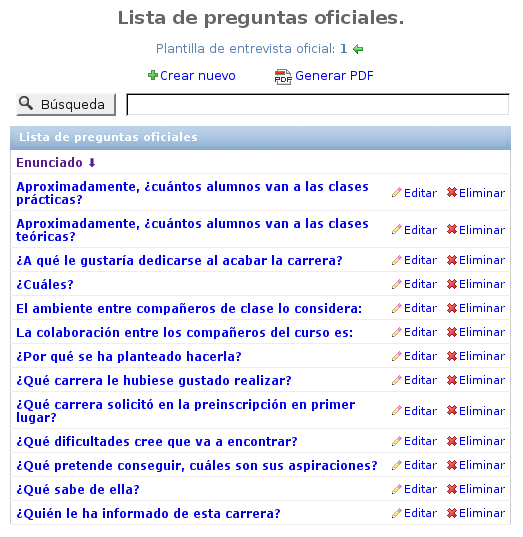
\includegraphics[scale=0.55]{4.Funcionamiento_Aplicacion/4.3.Gestion/4.3.1.Administrador_Principal/4.3.1.19.PreguntaOficial/lista_preguntas_oficiales.png}
      }
      \caption{Captura de pantalla de la lista de preguntas oficiales para el usuario \textit{Administrador principal}.}
      \label{capturaPantallaListaPreguntasOficialesAdminPrincipal}
    \end{center}
  \end{figure}
